\renewcommand{\thesection}{\arabic{section}}\renewcommand{\theHsection}{chapter.\arabic{section}}\setcounter{section}{11}\section{曲面积分}
\noindent\begin{minipage}{\textwidth}\ProblemHeading{例题}{12.1（改写）}
考虑半径与高都等于 $1$ 的直圆柱侧面。用包括上下底面所在平面的 $m+1$ 个等距水平面截得 $m+1$ 条圆周，并在每条圆周上取 $n$ 个等分点，其中 $m\ge1,n\ge3$。相邻圆周上的分点沿圆周方向错开圆心角 $\pi/n$；将每个分点与相邻圆周上距离它最近的两个分点连接，形成图示由 $2mn$ 个三角形组成的内接多面侧面，记其总面积为 $\sigma_{m,n}$。
\SubQ{1}{计算 $\sigma_{m,n}$。}
\SubQ{2}{当 $m,n\to\infty$ 且 $m/n^2\to q$（$0\le q<+\infty$）时，求 $\sigma_{m,n}$ 的极限。}
\SubQ{3}{当 $m,n\to\infty$ 且 $m/n^2\to+\infty$ 时，讨论 $\sigma_{m,n}$ 的行为。说明为何仅要求三角形的最大直径趋于零，不能保证内接多面侧面的面积趋于圆柱侧面积。}
\begin{center}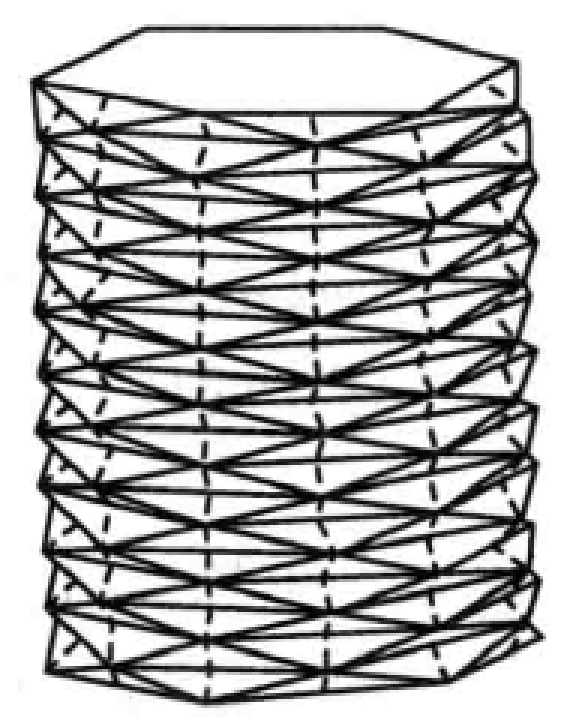
\includegraphics[width=0.28\linewidth]{figures/fig_12_1_1.png}\end{center}
\end{minipage}\par\vfill
\newpage
\noindent\begin{minipage}{\textwidth}\ProblemHeading{例题}{12.2}
计算半径 $a>0$ 的球面的面积。
\end{minipage}\par\vfill
\noindent\begin{minipage}{\textwidth}\ProblemHeading{例题}{12.3}
设 $a>0$。计算球面 $x^2+y^2+z^2=a^2$ 位于柱面 $x^2+y^2=ax$ 内部的部分的面积。
\end{minipage}\par\vfill
\noindent\begin{minipage}{\textwidth}\ProblemHeading{例题}{12.4}
设 $f\in C^1([a,b])$，且 $f\ge0$。求曲线 $y=f(x)$（$a\le x\le b$）绕 $x$ 轴旋转所得旋转曲面的面积公式。
\end{minipage}\par\vfill
\newpage
\noindent\begin{minipage}{\textwidth}\ProblemHeading{习题}{12.5（校订）}
计算下列曲面的面积，其中 $a>0$。
\SubQ{1}{锥面 $z=\sqrt{x^2+y^2}$ 被圆柱面 $x^2+y^2=2x$ 截下的内部部分。}
\SubQ{2}{圆柱面 $x^2+z^2=a^2$ 被圆柱面 $x^2+y^2=a^2$ 截下的内部部分。}
\SubQ{3}{圆柱面 $x^2+y^2=a^2$ 上介于平面 $x+z=0$ 与 $x-z=0$ 之间的有界部分，即 $-|x|\le z\le |x|$。}
\end{minipage}\par\vfill
\noindent\begin{minipage}{\textwidth}\ProblemHeading{习题}{12.6（校订）}
计算下列曲面的面积，其中 $a>0$。
\SubQ{1}{球面 $x^2+y^2+z^2=a^2$ 被椭圆柱面 $x^2/a^2+y^2/b^2=1$（$0<b\le a$）截下的内部部分。}
\SubQ{2}{马鞍面 $az=xy$ 被圆柱面 $x^2+y^2=a^2$ 截下的内部部分。}
\SubQ{3}{抛物面 $x^2+y^2=2az$ 被柱面 $(x^2+y^2)^2=2a^2xy$ 截下的内部部分。}
\end{minipage}\par\vfill
\noindent\begin{minipage}{\textwidth}\ProblemHeading{习题}{12.7（校订）}
计算下列曲面的面积，其中 $a>0$。
\SubQ{1}{螺旋面 $x=r\cos\theta,\ y=r\sin\theta,\ z=h\theta$（$0<r<a,\ 0\le\theta\le2\pi$）。}
\end{minipage}\par\vfill
\newpage
\noindent\begin{minipage}{\textwidth}\ProblemHeading{例题}{12.8}
计算 $\int_\Sigma(x+y+z)\,d\sigma$，其中 $\Sigma$ 为上半球面 $x^2+y^2+z^2=a^2,\ z\ge0$，$a>0$。
\end{minipage}\par\vfill
\noindent\begin{minipage}{\textwidth}\ProblemHeading{例题}{12.9}
设 $a>0$，$\Sigma$ 为球面 $x^2+y^2+z^2=a^2$。计算 $\int_\Sigma x^2\,d\sigma$，分别采用球坐标参数与对称性方法。
\end{minipage}\par\vfill
\noindent\begin{minipage}{\textwidth}\ProblemHeading{例题}{12.10}
设半径 $R>0$、球心位于原点的球面上均匀分布物质，面密度为 $1$。取万有引力常数为 $1$。求该球壳对球内及球外任意一点的引力场。
\end{minipage}\par\vfill
\newpage
\noindent\begin{minipage}{\textwidth}\ProblemHeading{习题}{12.11}
计算下列第一型曲面积分。
\SubQ{1}{$\displaystyle\int_\Sigma\frac{d\sigma}{(1+x+y)^2}$，$\Sigma$ 为四面体 $x+y+z\le1,\ x,y,z\ge0$ 的边界。}
\SubQ{2}{$\displaystyle\int_\Sigma|xyz|\,d\sigma$，$\Sigma:z=x^2+y^2,\ z\le1$。}
\SubQ{3}{$\displaystyle\int_\Sigma(xy+yz+zx)\,d\sigma$，$\Sigma$ 为锥面 $z=\sqrt{x^2+y^2}$ 在圆柱面 $x^2+y^2=2x$ 内的部分。}
\end{minipage}\par\vfill
\noindent\begin{minipage}{\textwidth}\ProblemHeading{习题}{12.12}
设 $\Sigma$ 为单位球面，$a,b,c$ 为常数，$f$ 在 $[-\sqrt{a^2+b^2+c^2},\sqrt{a^2+b^2+c^2}]$ 上连续。证明 Poisson 公式\[\int_\Sigma f(ax+by+cz)\,d\sigma=2\pi\int_{-1}^1 f\!\left(\sqrt{a^2+b^2+c^2}\,t\right)dt.\]
\end{minipage}\par\vfill
\noindent\begin{minipage}{\textwidth}\ProblemHeading{习题}{12.13}
设 $\Sigma(t)$ 为平面 $x+y+z=t$ 在单位球内的部分，$F(x,y,z)=1-(x^2+y^2+z^2)$。证明当 $|t|\le\sqrt3$ 时，\[\int_{\Sigma(t)}F\,d\sigma=\frac\pi{18}(3-t^2)^2.\]
\end{minipage}\par\vfill
\newpage
\noindent\begin{minipage}{\textwidth}\ProblemHeading{习题}{12.14（校订）}
设常数 $a,b,c$ 不全为零，$f$ 在 $[-\sqrt{a^2+b^2+c^2},\sqrt{a^2+b^2+c^2}]$ 上连续。证明\[\iiint_{x^2+y^2+z^2\le1}f\!\left(\frac{ax+by+cz}{\sqrt{x^2+y^2+z^2}}\right)dx\,dy\,dz=\frac{2\pi}{3}\int_{-1}^1 f\!\left(\sqrt{a^2+b^2+c^2}\,t\right)dt.\]原点处被积函数可任意补充一个有限值。
\end{minipage}\par\vfill
\noindent\begin{minipage}{\textwidth}\ProblemHeading{例题}{12.15（改写）}
把立方体的表面看作由六个正方形拼接成的曲面，在每一面上选择朝外的单位法向量。证明相邻两面在公共棱上诱导的边界方向相反，从而此拼接曲面可定向。
\end{minipage}\par\vfill
\noindent\begin{minipage}{\textwidth}\ProblemHeading{例题}{12.16（改写）}
矩形 $ABB_1A_1$ 被线段 $CD$ 分成两个小矩形，并按图示选择边界方向。将两端 $AB$ 与 $A_1B_1$ 粘合：分别考虑 $A\leftrightarrow A_1,B\leftrightarrow B_1$ 和 $A\leftrightarrow B_1,B\leftrightarrow A_1$ 两种方式。判断所得柱面与 Möbius 带能否取协调的定向，并说明理由。
\begin{center}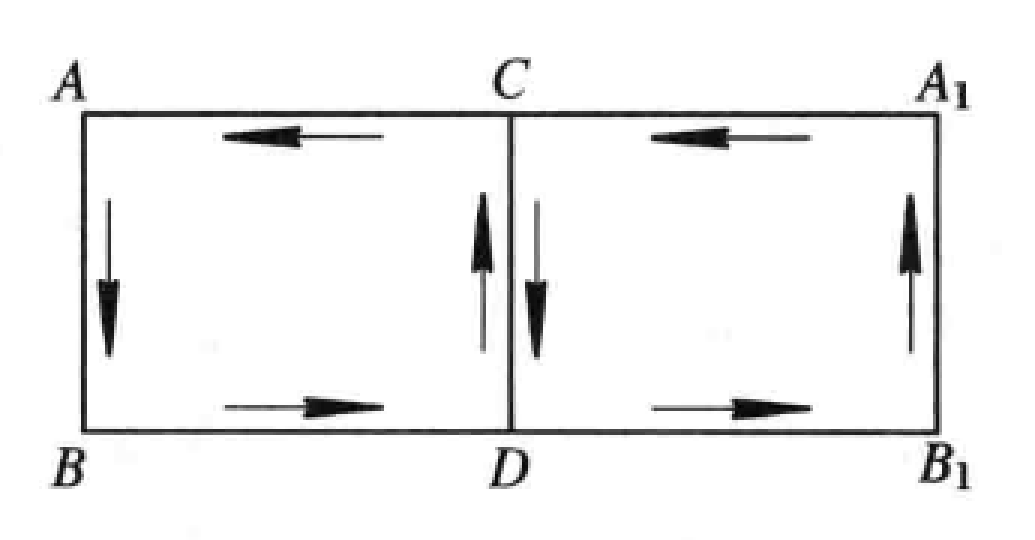
\includegraphics[width=0.48\linewidth]{figures/fig_12_16_1.png}\end{center}
\end{minipage}\par\vfill
\newpage
\noindent\begin{minipage}{\textwidth}\ProblemHeading{例题}{12.17}
计算第二型曲面积分 $\iint_\Sigma x\,dy\,dz+y\,dz\,dx+z\,dx\,dy$，其中 $\Sigma=\{(x,y,z):x,y,z\ge0,\ x+y+z=1\}$，法向量与 $(1,1,1)$ 同方向。
\end{minipage}\par\vfill
\noindent\begin{minipage}{\textwidth}\ProblemHeading{例题}{12.18}
设 $a>0$，$\Sigma$ 为球面 $x^2+y^2+z^2=a^2$ 的外侧。计算 $\iint_\Sigma x\,dy\,dz+y\,dz\,dx+z\,dx\,dy$。
\end{minipage}\par\vfill
\noindent\begin{minipage}{\textwidth}\ProblemHeading{例题}{12.19}
设流速场 $F=(yz,zx,xy)$，$\Sigma$ 为圆柱体 $x^2+y^2\le a^2,\ 0\le z\le h$ 的表面，其中 $a,h>0$。求流速场流出 $\Sigma$ 的总流量。
\end{minipage}\par\vfill
\newpage
\noindent\begin{minipage}{\textwidth}\ProblemHeading{例题}{12.20}
设 $a,b,c>0$，$\Sigma$ 为椭球面 $x^2/a^2+y^2/b^2+z^2/c^2=1$ 的外侧。计算 $\iint_\Sigma x^3\,dy\,dz+y^3\,dz\,dx+z^3\,dx\,dy$。
\end{minipage}\par\vfill
\noindent\begin{minipage}{\textwidth}\ProblemHeading{例题}{12.21}
设 $R>0$，$\Sigma$ 为球面 $(x-a)^2+(y-b)^2+(z-c)^2=R^2$ 的外侧。计算 $\iint_\Sigma x^2\,dy\,dz+y^2\,dz\,dx+z^2\,dx\,dy$。
\end{minipage}\par\vfill
\noindent\begin{minipage}{\textwidth}\ProblemHeading{习题}{12.22}
计算下列第二型曲面积分，其中 $a,b,c,h>0$，出现的函数连续。
\SubQ{1}{$\displaystyle\iint_\Sigma x^4\,dy\,dz+y^4\,dz\,dx+z^4\,dx\,dy$，$\Sigma:x^2+y^2+z^2=a^2$，取内侧。}
\SubQ{2}{$\displaystyle\iint_\Sigma xz\,dy\,dz+yz\,dz\,dx+x^2\,dx\,dy$，$\Sigma:x^2+y^2+z^2=a^2$，取外侧。}
\SubQ{3}{$\displaystyle\iint_\Sigma f(x)\,dy\,dz+g(y)\,dz\,dx+h(z)\,dx\,dy$，$\Sigma$ 为 $[0,a]\times[0,b]\times[0,c]$ 的边界，取外侧。}
\end{minipage}\par\vfill
\newpage
\noindent\begin{minipage}{\textwidth}\ProblemHeading{习题}{12.23}
计算下列第二型曲面积分，其中 $a,b,c,h>0$，出现的函数连续。
\SubQ{1}{$\displaystyle\iint_\Sigma z\,dx\,dy$，$\Sigma:x^2/a^2+y^2/b^2+z^2/c^2=1$，取外侧。}
\SubQ{2}{$\displaystyle\iint_\Sigma(y-z)\,dy\,dz+(z-x)\,dz\,dx+(x-y)\,dx\,dy$，$\Sigma:z=\sqrt{x^2+y^2},\ z\le h$，取外侧。}
\end{minipage}\par\vfill
\noindent\begin{minipage}{\textwidth}\ProblemHeading{习题}{12.24}
设流速场 $F=(y,z,x)$。计算它流出圆柱体 $x^2+y^2\le R^2,\ 0\le z\le h$ 的闭合表面的总流量，其中 $R,h>0$。
\end{minipage}\par\vfill
\noindent\begin{minipage}{\textwidth}\ProblemHeading{习题}{12.25}
设 $\Sigma:z=f(x,y)$（$(x,y)\in D$）取向上的法向量，$f\in C^1$，$P,Q$ 连续。证明：
\SubQ{1}{$\displaystyle\iint_\Sigma P\,dy\,dz=-\iint_D P(x,y,f(x,y))\frac{\partial f}{\partial x}\,dx\,dy$。}
\SubQ{2}{$\displaystyle\iint_\Sigma Q\,dz\,dx=-\iint_D Q(x,y,f(x,y))\frac{\partial f}{\partial y}\,dx\,dy$。}
\end{minipage}\par\vfill
\newpage
\noindent\begin{minipage}{\textwidth}\ProblemHeading{例题}{12.26}
利用 Gauss 公式计算 $\iint_\Sigma x\,dy\,dz+y\,dz\,dx+z\,dx\,dy$，其中 $\Sigma$ 为半径 $a>0$、球心在原点的球面，取外侧。
\end{minipage}\par\vfill
\noindent\begin{minipage}{\textwidth}\ProblemHeading{例题}{12.27}
利用 Gauss 公式计算 $\iint_\Sigma x\,dy\,dz+y\,dz\,dx+z\,dx\,dy$，其中 $\Sigma=\{(x,y,z):x,y,z\ge0,\ x+y+z=1\}$，法向量与 $(1,1,1)$ 同向。
\end{minipage}\par\vfill
\noindent\begin{minipage}{\textwidth}\ProblemHeading{例题}{12.28}
证明 Archimedes 原理：物体全部浸入密度为常数 $\rho$ 的静止液体中时，所受浮力等于与物体同体积液体的重量。假设重力加速度 $g$ 恒定，物体表面分段光滑。
\end{minipage}\par\vfill
\newpage
\noindent\begin{minipage}{\textwidth}\ProblemHeading{例题}{12.29}
设有向曲面 $\Sigma:x+y+z=1,\ x,y,z\ge0$ 的法向量与 $(1,1,1)$ 同方向。求力场 $F=(y^2,z^2,x^2)$ 绕 $\Sigma$ 的正向边界 $\partial\Sigma$ 一周所做的功。
\end{minipage}\par\vfill
\noindent\begin{minipage}{\textwidth}\ProblemHeading{例题}{12.30（校订）}
设 $0<b<a$，$\Gamma$ 为曲面 $x^2+y^2+z^2=2ax$ 与 $x^2+y^2=2bx$ 在 $z\ge0$ 中的交线，取其在 $xy$ 平面上的正射影从 $z$ 轴正半轴观察时沿逆时针绕行的方向。计算\[\int_\Gamma(y^2+z^2)\,dx+(z^2+x^2)\,dy+(x^2+y^2)\,dz.\]
\end{minipage}\par\vfill
\noindent\begin{minipage}{\textwidth}\ProblemHeading{习题}{12.31}
利用 Gauss 公式计算下列积分，其中 $R>0$。
\SubQ{1}{$\displaystyle\iint_\Sigma x^2\,dy\,dz+y^2\,dz\,dx+z^2\,dx\,dy$，$\Sigma:x^2+y^2+z^2=R^2$，方向朝外。}
\SubQ{2}{$\displaystyle\iint_\Sigma xy\,dy\,dz+yz\,dz\,dx+zx\,dx\,dy$，$\Sigma$ 为平面 $x=0,y=0,z=0,x+y+z=1$ 围成的闭合曲面，方向朝外。}
\SubQ{3}{$\displaystyle\iint_\Sigma(x-y)\,dy\,dz+(y-z)\,dz\,dx+(z-x)\,dx\,dy$，$\Sigma:z=x^2+y^2,\ z\le1$，方向朝下。}
\end{minipage}\par\vfill
\newpage
\noindent\begin{minipage}{\textwidth}\ProblemHeading{习题}{12.32}
利用 Gauss 公式计算下列积分，其中 $R>0$。
\SubQ{1}{$\displaystyle\iint_\Sigma x^2\,dy\,dz+y^2\,dz\,dx+z^2\,dx\,dy$，$\Sigma:z^2=x^2+y^2,\ 0\le z\le1$，方向朝下。}
\end{minipage}\par\vfill
\noindent\begin{minipage}{\textwidth}\ProblemHeading{习题}{12.33}
设 $\Omega$ 为有界闭区域，边界分段光滑，$\mathbf n$ 为其单位外法向量，$\mathbf e$ 为固定非零向量。证明 $\int_{\partial\Omega}\cos\angle(\mathbf e,\mathbf n)\,d\sigma=0$。
\end{minipage}\par\vfill
\noindent\begin{minipage}{\textwidth}\ProblemHeading{习题}{12.34}
设 $\Omega$ 为有界闭区域，边界分段光滑，$\mathbf n$ 为单位外法向量，$(a,b,c)\notin\partial\Omega$。令 $\mathbf p=(x-a,y-b,z-c)$、$p=\|\mathbf p\|$。证明\[\iiint_\Omega\frac{dx\,dy\,dz}{p}=\frac12\int_{\partial\Omega}\cos\angle(\mathbf p,\mathbf n)\,d\sigma.\]若 $(a,b,c)\in\Omega$，体积分按反常积分理解。
\end{minipage}\par\vfill
\newpage
\noindent\begin{minipage}{\textwidth}\ProblemHeading{习题}{12.35}
利用 Stokes 公式计算下列积分，其中 $a>0$。
\SubQ{1}{$\displaystyle\int_\Gamma y\,dx+z\,dy+x\,dz$，$\Gamma:x^2+y^2+z^2=a^2,\ x+y+z=0$，从第一卦限看去沿逆时针方向。}
\SubQ{2}{$\displaystyle\int_\Gamma(y+z)\,dx+(z+x)\,dy+(x+y)\,dz$，$\Gamma:x^2+y^2=2y,\ y=z$，从 $(0,1,0)$ 向 $\Gamma$ 看去沿逆时针方向。}
\SubQ{3}{$\displaystyle\int_\Gamma y^2\,dx+z^2\,dy+x^2\,dz$，$\Gamma:x^2+y^2+z^2=a^2,\ x+y+z=a$，从原点看去沿逆时针方向。}
\end{minipage}\par\vfill
\noindent\begin{minipage}{\textwidth}\ProblemHeading{习题}{12.36}
设有向曲面 $\Sigma$ 的单位法向量为 $\mathbf n$，边界方向与曲面方向协调，$\mathbf a$ 为常向量，$\mathbf p=(x,y,z)$。证明\[\int_{\partial\Sigma}(\mathbf a\times\mathbf p)\cdot d\mathbf p=2\iint_\Sigma\mathbf a\cdot\mathbf n\,d\sigma.\]
\end{minipage}\par\vfill
\noindent\begin{minipage}{\textwidth}\ProblemHeading{习题}{12.37}
计算 $\int_\Gamma y\,dx+z\,dy+x\,dz$，其中 $\Gamma$ 为平面 $x+y=2$ 与球面 $x^2+y^2+z^2=2(x+y)$ 的交圆，从原点看去顺时针方向为正向。
\end{minipage}\par\vfill
\newpage
\noindent\begin{minipage}{\textwidth}\ProblemHeading{习题}{12.38}
计算 $\int_\Gamma y\,dx+z\,dy+x\,dz$，其中 $\Gamma$ 为 $z=xy$ 与 $x^2+y^2=1$ 的交线；沿 $\Gamma$ 的正向行进时，$z$ 轴在左手边。
\end{minipage}\par\vfill
\noindent\begin{minipage}{\textwidth}\ProblemHeading{习题}{12.39（校订）}
设 $a>0$，定向曲线 $\Gamma:x^2+y^2+z^2=a^2,\ x^2+y^2=ax,\ z\ge0$，取其在 $xy$ 平面上的正射影从 $z$ 轴正半轴观察时沿逆时针绕行的方向。计算力场 $F=(y^2,z^2,x^2)$ 沿 $\Gamma$ 所做的功。
\end{minipage}\par\vfill
\noindent\begin{minipage}{\textwidth}\ProblemHeading{习题}{12.40}
质量为 $m$ 的质点在力场 $F$ 作用下沿曲线 $\Gamma$ 从 $\mathbf a$ 运动到 $\mathbf b$，速度向量记为 $\mathbf v$，并满足 Newton 第二定律。证明\[\int_\Gamma F\cdot d\mathbf p=\frac m2\bigl(\|\mathbf v(\mathbf b)\|^2-\|\mathbf v(\mathbf a)\|^2\bigr).\]
\end{minipage}\par\vfill
\newpage
\noindent\begin{minipage}{\textwidth}\ProblemHeading{例题}{12.41}
设微分形式 $\omega=f\,dx+g\,dy+h\,dz$，$\theta=P\,dx+Q\,dy+R\,dz$。计算 $\omega\wedge\theta$。
\end{minipage}\par\vfill
\noindent\begin{minipage}{\textwidth}\ProblemHeading{例题}{12.42}
设微分形式 $\omega=f\,dx+g\,dy+h\,dz$，$\theta=P\,dy\wedge dz+Q\,dz\wedge dx+R\,dx\wedge dy$。计算 $\omega\wedge\theta$。
\end{minipage}\par\vfill
\noindent\begin{minipage}{\textwidth}\ProblemHeading{习题}{12.43}
计算下列微分形式的外积。
\SubQ{1}{$(x\,dx+y\,dy)\wedge(z\,dz-z\,dx)$。}
\SubQ{2}{$(dx+dy+dz)\wedge(x\,dx\wedge dy-z\,dy\wedge dz)$。}
\end{minipage}\par\vfill
\newpage
\noindent\begin{minipage}{\textwidth}\ProblemHeading{习题}{12.44}
计算 $d\omega$。
\SubQ{1}{$\omega=xy+yz+zx$。}
\SubQ{2}{$\omega=xy\,dx$。}
\SubQ{3}{$\omega=(xy+yz)\,dx$。}
\end{minipage}\par\vfill
\noindent\begin{minipage}{\textwidth}\ProblemHeading{习题}{12.45}
计算 $d\omega$。
\SubQ{1}{$\omega=xy\,dx+x^2\,dy$。}
\SubQ{2}{$\omega=x^2y\,dx-yze^x\,dy$。}
\SubQ{3}{$\omega=xy^2\,dy\wedge dz-xz^2\,dx\wedge dy$。}
\end{minipage}\par\vfill
\noindent\begin{minipage}{\textwidth}\ProblemHeading{习题}{12.46}
计算 $d\omega$。
\SubQ{1}{$\omega=xy\,dy\wedge dz+yz\,dz\wedge dx+zx\,dx\wedge dy$。}
\end{minipage}\par\vfill
\newpage
\noindent\begin{minipage}{\textwidth}\ProblemHeading{习题}{12.47}
设微分形式 $\omega$ 的系数函数属于 $C^2$。证明 $d(d\omega)=0$。
\end{minipage}\par\vfill
\noindent\begin{minipage}{\textwidth}\ProblemHeading{习题}{12.48}
考虑 $\mathbb R^n$ 中 $n$ 个一次微分形式 $\omega_j=\sum_{i=1}^n a_i^j(x)\,dx_i$（$j=1,\ldots,n$）。证明\[\omega_1\wedge\cdots\wedge\omega_n=\det(a_i^j(x))\,dx_1\wedge\cdots\wedge dx_n.\]
\end{minipage}\par\vfill
\noindent\begin{minipage}{\textwidth}\ProblemHeading{习题}{12.49}
设 $f_1,\ldots,f_n$ 为 $\mathbb R^n$ 上的 $C^1$ 数量函数。证明\[df_1\wedge\cdots\wedge df_n=\frac{\partial(f_1,\ldots,f_n)}{\partial(x_1,\ldots,x_n)}\,dx_1\wedge\cdots\wedge dx_n.\]
\end{minipage}\par\vfill
